%   % !TEX root = ../../VIII,3_Rahmen-TeX_9-0.tex
%  
%   Band VIII, 3 N.~?? 	Stoß
%   Signatur/Tex-Datei:	LH_37_05_140-141,148-149
%
%   RK-Nr. 	57275
%
%   Überschrift: 	(keine)	
%   Titel: 			??			(unser Titel)					??
%   Datierung:		???? bis ???? (a. St.?), eigh. (?)				??
%   Textfolge: 					(ggf. wie Foliierung)				??
%   WZ: 			keins
%   edlabels:			12
%   Diagramme: 		9 + 1 (auf Träger 148-149)
%   Dateien (PDF): [veraltet]
%   		LH_37_05_140-141_d1_140r
%   		LH_37_05_140-141_d2_140r
%   		LH_37_05_140-141_d3_140v	(gestr.)
%   		LH_37_05_140-141_d4_141r
%   		LH_37_05_140-141_d5_141r
%   		LH_37_05_140-141_d6_141r
%   		LH_37_05_140-141_d7_141v
%   		LH_37_05_140-141_d8_141v
%   		LH_37_05_140-141_d9_141v (wird nicht benutzt?)
%   		LH_37_05_140-141_d9b_141v ??? 10???
%
%   Erstaufnahme:			(wer?)
%   Bearbeitung MS ab: 		Mai 2020
%
%   NB: 		Diagramm 1 befindet sich auf Bl. 149r
%
%
%
%
%
\selectlanguage{ngerman}
\frenchspacing
%
\begin{ledgroupsized}[r]{120mm}
\footnotesize
\pstart
\noindent\textbf{Überlieferung:}
\pend
\end{ledgroupsized}
%
\begin{ledgroupsized}[r]{114mm}
\footnotesize
\pstart \parindent -6mm
\makebox[6mm][l]{\textit{L}}%
Konzept:
LH~XXXVII~5~Bl.~140\textendash141, 148\textendash149. 
Zwei Bögen~4\textsuperscript{o};
Bl.~148 ist halbiert; Wasserzeichenfragment im Falz von Bl.~148\textendash149;
Ränder ausgefranst; Papiererhaltungsmaßnahmen.
Ein Diagramm (\lbrack\textit{Fig.~1}\rbrack) im oberen Bereich von \lbrack149~r\textsuperscript{o}\rbrack\
und vier Seiten auf Bl.~140\textendash141;
Bl.~148\textendash149 überliefert auch N.~\ref{RK57276}.
\pend
\end{ledgroupsized}
%
\begin{ledgroupsized}[r]{114mm}
\footnotesize
\pstart
\parindent -6mm
\makebox[6mm][l]{\textit{E}}%
(tlw.) \textsc{Fichant} 1994, S.~394\cite{01056}.
\pend%
\end{ledgroupsized}
%
%
\vspace{5mm}
\begin{ledgroup}
\footnotesize
\pstart
\noindent%
\textbf{Datierungsgründe:} %
Im vorliegenden Konzept geht Leibniz, wie bereits in N.~\ref{RK57273}, N.~\ref{RK57274} und N.~\ref{RK57277},
%
von der These der gleichförmigen Bewegung des \textit{centrum potentiae} zweier Körper beim Stoß aus.
%
Aus ihr heraus möchte Leibniz die drei möglichen Fälle des Stoßes eines Körpers auf einen zweiten ruhenden bestimmen.
%
Jedoch erweist sich nach einer eingehenden Fallanalyse die These selbst als nicht haltbar 
%
(\glqq Casus 3.\ ostendit generalitatem principii nostri esse impossibilem\grqq, S.~\refpassage{37_05_140-141_13a}{37_05_140-141_13b})
%
und Leibniz sieht sich zur Aufgabe der angeblichen Gesetzmäßigkeit gezwungen.
%
Im Anschluss daran untersucht er die These der gleichförmigen Bewegung des Schwerpunkts (\textit{centrum gravitatis}) 
%
und findet sie in allen drei Fällen bestätigt. 
%
Daraufhin bespricht er in einer \glqq Nota\grqq\ (S.~\refpassage{37_05_140-141_15a}{37_05_140-141_15b}) 
die Übereinstimmung der letzteren Gesetzmäßigkeit  mit seinem Ansatz, 
%
die Stoßphänomene anhand der Schiffsmethode und des Relativitätsprinzips
(das er außerdem auf S.~\refpassage{37_05_140-141_14a}{37_05_140-141_14b} formuliert) zu analysieren.
%
Leibniz hatte die Schiffsanalogie zur Analyse des Stoßes in N.~\ref{RK57269} vom 10.\ (20.) Juni 1677 eingeführt, das damit einen Terminus post quem für die Entstehung von  N.~\ref{RK57275} abgibt.
%
Auch muss das Konzept nach den obengenannten Stücken, die sich auf die hier für ungültig erklärte These der gleichförmigen Bewegung des \textit{centrum potentiae} stützten, entstanden sein;
%
darunter ist N.~\ref{RK57277}, dessen Entstehung nach N.~\ref{RK57269} unabhängig festgestellt werden kann (siehe die Datierungsgründe).
\pend
%
\pstart
Als Terminus ante quem darf  \textit{De corporum concursu}, \textit{Scheda octava} von Januar 1678 (N.~\ref{dcc_08}) gelten.
%
Denn Leibniz sieht in N.~\ref{RK57275}, wie bereits in N.~\ref{RK57276}, das Hauptproblem seiner Methode und der
%
daraus fließenden (und aus heutiger Sicht grundsätzlich richtigen) Stoßregel darin, dass 
%
sie die Erhaltung der gesamten \textit{potentia} der Körper wider Erwarten nicht gewährleistet
(S.~\refpassage{37_05_140-141_7a}{37_05_140-141_7b}).
%
Der Grund dafür ist, dass er unter \textit{potentia} die skalare Größe $mv$ versteht, die im Gegensatz zum (vektoriellen) Impuls  beim Stoß nicht erhalten wird.
%
In der \textit{Scheda octava} wird Leibniz eine \glqq reformatio\grqq\  der Stoßlehre vollziehen,
%
die Erhaltungssätze für den Impuls und für die dort erstmals als $mv^2$ gemessene \textit{vis} umfasst,
%
wodurch die in N.~\ref{RK57275} (und N.~\ref{RK57276}) geäußerten Bedenken über die Nichterhaltung der Bewegungsgröße sich als gegenstandslos erweisen.
%
Die quadratische Gleichung der Passage auf S.~\refpassage{37_05_140-141_12a}{37_05_140-141_12b}, 
(die auch in N.~\ref{RK57273} und N.~\ref{RK60344_2} ausführlich berechnet worden war),
%
kann dabei als Vorgängerin der \glqq aequatio infallibilis\grqq\ der \textit{Scheda octava}
(S.~\refpassage{LH_37_05_086r_aequatioinfall-1}{LH_37_05_086r_aequatioinfall-1}) angesehen werden.
\pend
%
\pstart
Die thematischen und inhaltlichen Übereinstimmungen zwischen N.~\ref{RK57275} und N.~\ref{RK57276} 
legen die Annahme einer etwa gleichzeitigen Entstehung beider Stücke nahe,
%
welche durch folgenden Umstand bestätigt und präzisiert wird.
%
Die Stoßanalyse anhand der Bewegung des \textit{centrum potentiae} (und später der Schwerpunkts) zu Beginn von N.~\ref{RK57275} 
%
gliedert sich in die Besprechungen dreier Stoßfälle, die Leibniz allerdings nirgends ausdrücklich formuliert oder beschreibt.
%
Er muss sich dabei an der dreiteiligen Figur \lbrack\textit{Fig.~1}\rbrack\ orientiert haben, die alle Eigenschaften der drei Fälle
%
abbildet und dem Text von N.~\ref{RK57275} genau entspricht.
%
Die Zeichnung befindet sich allerdings nicht auf demselben Träger wie der Text von N.~\ref{RK57275},
%
sondern auf einem anderen Bogen, der hauptsächlich N.~\ref{RK57276} überliefert, im oberen Bereich von Bl.~149~r\textsuperscript{o}.
%
Die Lage der Figur lässt den Schluss zu, dass Leibniz nach Anfertigung von N.~\ref{RK57276} 
%
sie am frei gebliebenen Rand von Bl.~149~r\textsuperscript{o} zeichnete und anschließend
%
zur Abfassung von N.~\ref{RK57275} ansetzte.
\pend
%
\end{ledgroup}
%
%
\selectlanguage{latin}
\frenchspacing
% \newpage%
\vspace{8mm}
\pstart%
\normalsize%
\noindent%
\edtext{\lbrack149~r\textsuperscript{o}\rbrack}{%
\lemma{\hspace*{1,6mm}%
\lbrack\textit{Fig.~1}\rbrack%	%
}\killnumber%
\Cfootnote{%
Leibniz hat im Fall (3) die Punktbezeichnung \textit{{\scriptsize 3}C} nachträglich gestrichen sowie den Punkt \textit{{\scriptsize 3}B}, der zunächst mit \textit{{\scriptsize 1}G} zusammenfiel, nachträglich verlegt.}}
\pend
%
\vspace{1.0em} %%%%%%%%% Diagramm 1
\centerline{%
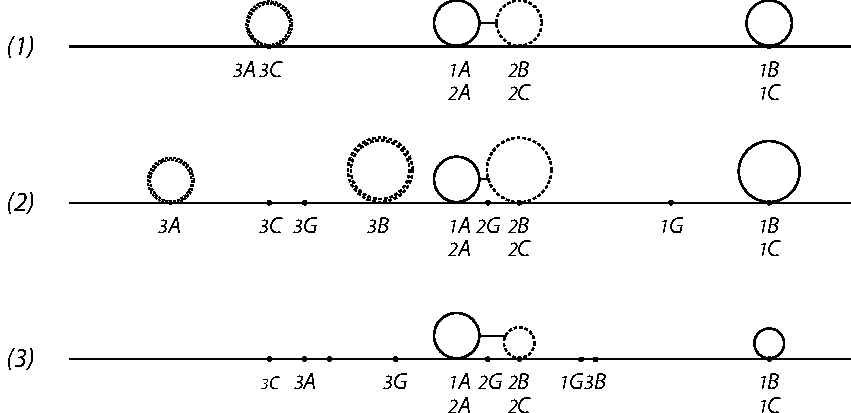
\includegraphics[width=1\textwidth]{%
gesamttex/edit_VIII,3/images/LH_37_05_140-141,148-149_d1_149r.pdf%
}} 
\vspace{0.5em}
\centerline{%
\lbrack\textit{Fig.~1}\rbrack}
% \newpage%
\vspace{1em}
%
\pstart%
\lbrack140~r\textsuperscript{o}\rbrack\
Casus 1.\ demonstratur: nam centrum 
%
\edtext{potentiae\protect\index{Sachverzeichnis}{centrum potentiae} non}{\lemma{potentiae}\Bfootnote{\textit{(1)}~necessario \textit{(2)}~non~\textit{L}}} 
%
potest esse celerius 
%
\edtext{corpore versus}{\lemma{corpore}\Bfootnote{\textit{(1)}~quod \textit{(2)}~versus~\textit{L}}} 
%
cujus partem tendit, nec tardius corpore quod ipsum sequitur; alioqui durante diu motu illud praecurreret aut ab hoc praecurreretur, nec proinde esset in medio. 
%
Ergo cum motus centri potentiae\protect\index{Sachverzeichnis}{centrum potentiae}\protect\index{Sachverzeichnis}{motus centri potentiae} 
%
in casu praecedenti
%
idem fuerit cum motu corporis \textit{B}, usque ad \protect\index{Sachverzeichnis}{concursus}concursum, non potest post concursum celeritas illa  dividi in duo corpora \textit{A} et \textit{B}, nam pars quam acciperet \textit{A}, foret minor toto, ergo minor celeritate centri gravitatis\protect\index{Sachverzeichnis}{celeritas centri gravitatis} quod est absurdum.
%
\edtext{Nam \textit{A}}{\lemma{}\Bfootnote{Nam \textbar\ ita \textit{gestr.}~\textbar\ \textit{A}~\textit{L}}} 
%
est corpus quod \textit{C} praecedit seu in cujus partem \textit{C} tendit. Ergo necesse est \textit{C} totam accipiat celeritatem. Q.~E.~D. 
%
\pend \pstart
%
In casu 
%
\edtext{2\textsuperscript{do} ubi}{\lemma{2\textsuperscript{do}}\Bfootnote{\textit{(1)}~necessario \textit{(2)}~ubi~\textit{L}}} 
%
corpus majus\protect\index{Sachverzeichnis}{corpus majus} incurrit in minor quiescens\protect\index{Sachverzeichnis}{corpus minus quiescens}, necessario et minus\protect\index{Sachverzeichnis}{corpus minus} et majus procedit. Nam quia \textit{C} procedit ex \textit{\scriptsize 2}\textit{C} in \textit{\scriptsize 3}\textit{C}, necessario et \textit{\scriptsize 3}\textit{A} minimum procedet tantundem, sed si \textit{\scriptsize 3}\textit{A} tantum 
%
\edtext{procederet tantundem, et \textit{B}}{\lemma{procederet tantundem,}\Bfootnote{\textit{(1)}~tunc \textit{\scriptsize 2}\textit{C} et \textit{(2)}~et \textit{B}~\textit{L}}} 
%
quiesceret seu \textit{\scriptsize 3}\textit{B} coincideret \textit{\scriptsize 2}\textit{B}\lbrack,\rbrack\ tunc minor esset potentia\protect\index{Sachverzeichnis}{potentia} quam ante, ergo necesse esset \textit{\scriptsize 3}\textit{B} procedere (\protect\vphantom)nam non regreditur, quia cum aequale non repellatur\lbrack,\rbrack\ 
%
\edtext{ex praecedenti casu\lbrack,\rbrack}{\lemma{}\Bfootnote{ex praecedenti casu \textit{erg.~L}}} 
%
multo minus majus\protect\vphantom(). Hinc patet etiam \textit{\scriptsize 3}\textit{C} et \textit{\scriptsize 3}\textit{A} non coincidere, quia ambo progrediuntur.
%
Tantum superest ut determinemus rectas: \textit{\scriptsize 2}\textit{A}\textit{\scriptsize 3}\textit{A}, et \textit{\scriptsize 2}\textit{B}\textit{\scriptsize 3}\textit{B}. \pend
%
\pstart\noindent
Est autem: 
%
\textit{\scriptsize 2}\textit{A}\textit{\scriptsize 3}$A \smallfrown \raisebox{-1.0ex}{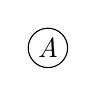
\begin{tikzpicture}\draw (0,0) circle (0.25cm) node {\textit{A}};\end{tikzpicture}}%
+ {\scriptstyle \textit{2}}B{\scriptstyle \textit{3}}B \smallfrown \raisebox{-1.0ex}{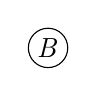
\begin{tikzpicture}\draw (0,0) circle (0.25cm) node {\textit{B}};\end{tikzpicture}}\; \sqcap$ datae potentiae, \textit{p}. \pend
%
\pstart\noindent
%
Et $\displaystyle\frac{{\scriptstyle \textit{3}}B{\scriptstyle \textit{3}}C}{{\scriptstyle \textit{3}}A{\scriptstyle \textit{3}}C} \sqcap \displaystyle\frac{{\scriptstyle \textit{2}}A{\scriptstyle \textit{3}}A \smallfrown\raisebox{-1.0ex}{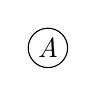
\begin{tikzpicture}\draw (0,0) circle (0.25cm) node {\textit{A}};\end{tikzpicture}}}{{\scriptstyle \textit{2}}B{\scriptstyle \textit{3}}B \smallfrown \raisebox{-1.0ex}{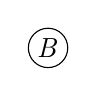
\begin{tikzpicture}\draw (0,0) circle (0.25cm) node {\textit{B}};\end{tikzpicture}}}$\rule[-8mm]{0pt}{15mm}.\pend
%
\pstart\noindent
%
${\scriptstyle \textit{2}}C{\scriptstyle \textit{3}}C \sqcap {\scriptstyle \textit{2}}C{\scriptstyle \textit{2}}B+{\scriptstyle \textit{2}}B{\scriptstyle \textit{3}}B+{\scriptstyle \textit{3}}B{\scriptstyle \textit{3}}C$.\pend
%
\pstart\noindent
$\phantom{\;{\scriptstyle \textit{2}}C{\scriptstyle \textit{3}}\;} (\sqcap$) ${\scriptstyle \textit{2}}C{\scriptstyle \textit{2}}A+{\scriptstyle \textit{2}}A{\scriptstyle \textit{3}}A-{\scriptstyle \textit{3}}A{\scriptstyle \textit{3}}C$. 
\pend
%
\pstart\noindent
Ergo pro quatuor incognitis nempe \textit{{\scriptsize 2}A{\scriptsize 3}A}, \textit{{\scriptsize 2}B{\scriptsize 3}B},
%
\edtext{\lbrack\textit{{\scriptsize 3}}\rbrack\textit{B{\scriptsize 3}C},}{%
\lemma{}%
\Bfootnote{%
\textit{{\scriptsize 2}B{\scriptsize 3}C} %
\textit{L ändert Hrsg.}%
}}
%
\textit{{\scriptsize 3}A{\scriptsize 3}C},
habemus 4 aequationes quod sufficit, et fiet
\pend
%
\pstart\noindent
\protect\rule[0cm]{0mm}{16pt}\textit{{\scriptsize2}C{\scriptsize2}A} \raisebox{-1.5ex}{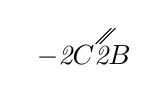
\begin{tikzpicture} \draw (.15,.15) -- (.35,.35); \draw (.2,.15) -- (.4,.35); \node[draw=none,fill=none] {\ovalbox{$-{\scriptstyle \textit{2}}C{\scriptstyle \textit{2}}B$}}; \end{tikzpicture}} $\sqcap$ \raisebox{-1.5ex}{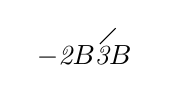
\begin{tikzpicture} \draw (.2,.15) -- (.4,.35); \node[draw=none,fill=none] {\ovalbox{$-{\scriptstyle \textit{2}}B{\scriptstyle \textit{3}}B$}}; \end{tikzpicture}} \ovalbox{\ovalbox{$+{\scriptstyle \textit{3}}B{\scriptstyle \textit{3}}C \sqcap$}} \textit{{\scriptsize2}C{\scriptsize3}C} \raisebox{-1.5ex}{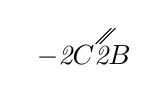
\begin{tikzpicture} \draw (.15,.15) -- (.35,.35); \draw (.2,.15) -- (.4,.35); \node[draw=none,fill=none] {\ovalbox{$-{\scriptstyle \textit{2}}C{\scriptstyle \textit{2}}B$}}; \end{tikzpicture}} \raisebox{-1.5ex}{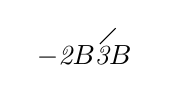
\begin{tikzpicture} \draw (.2,.15) -- (.4,.35); \node[draw=none,fill=none] {\ovalbox{$-{\scriptstyle \textit{2}}B{\scriptstyle \textit{3}}B$}}; \end{tikzpicture}}\\
%
%
\rule[-0mm]{30.5mm}{0mm}\raisebox{-6.25ex}{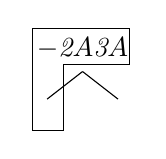
\begin{tikzpicture} \draw (-0.64,0.25) -- (-0.64,-1.05); \draw (-0.64,0.25) -- (0.6,.25); \draw (0.6,0.25) -- (0.6,-0.21); \draw (-0.24,-0.21) -- (0.6,-0.21); \draw (-0.64,-1.05) -- (-0.24,-1.05); \draw (-0.24,-0.21) -- (-0.24,-1.05);  \node[draw=none,fill=none] {$-{\scriptstyle \textit{2}}A{\scriptstyle \textit{3}}A$}; \draw (0.0,-.3) -- (-0.45,-0.65); \draw (0.0,-.3) -- (.45,-0.65); \end{tikzpicture}} 
%\rule[-0mm]{30.5mm}{0mm}\raisebox{-6.25ex}{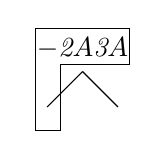
\begin{tikzpicture} \draw (-0.6,0.25) -- (-0.6,-1.05); \draw (-0.6,0.25) -- (0.6,.25); \draw (0.6,0.25) -- (0.6,-0.21); \draw (-0.28,-0.21) -- (0.6,-0.21); \draw (-0.6,-1.05) -- (-0.28,-1.05); \draw (-0.28,-0.21) -- (-0.28,-1.05);  \node[draw=none,fill=none] {$-{\scriptstyle \textit{2}}A{\scriptstyle \textit{3}}A$}; \draw (0.0,-.3) -- (-0.45,-0.75); \draw (0.0,-.3) -- (.45,-0.75); \end{tikzpicture}} 
%
\ovalbox{$+{\scriptstyle \textit{3}}A{\scriptstyle \textit{3}}C \sqcap$} $\displaystyle\frac{{\scriptstyle \textit{2}}B{\scriptstyle \textit{3}}B}{{\scriptstyle \textit{2}}A{\scriptstyle \textit{3}}A} \smallfrown \displaystyle\frac{\raisebox{-1.0ex}{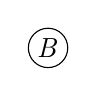
\begin{tikzpicture}\draw (0,0) circle (0.25cm) node {\textit{B}};\end{tikzpicture}}}{\raisebox{-1.0ex}{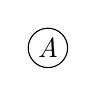
\begin{tikzpicture}\draw (0,0) circle (0.25cm) node {\textit{A}};\end{tikzpicture}}}$ \ovalbox{\ovalbox{\textit{{\scriptsize3}B{\scriptsize3}C}}} \quad$=\overline{{\scriptstyle \textit{2}}C{\scriptstyle \textit{3}}C-{\scriptstyle \textit{2}}C{\scriptstyle \textit{2}}B-{\scriptstyle \textit{2}}B{\scriptstyle \textit{3}}B}$ 
%
\pend \vspace{-4ex} 
%
\pstart\noindent  
\rule[-0mm]{31mm}{0mm}$\displaystyle\efrac{\sqcap}{}$ $-\displaystyle\frac{p-{\scriptstyle \textit{2}}B{\scriptstyle \textit{3}}B\;\raisebox{-1.0ex}{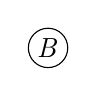
\begin{tikzpicture}\draw (0,0) circle (0.25cm) node {\textit{B}};\end{tikzpicture}}}{\raisebox{-1.0ex}{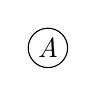
\begin{tikzpicture}\draw (0,0) circle (0.25cm) node {\textit{A}};\end{tikzpicture}}}$\hfill
\pend
%
\pstart\noindent
\protect\rule[0cm]{0mm}{12pt}Habetur ergo valor ipsius \textit{{\scriptsize 2}B{\scriptsize 3}B}. 
\pend
\pstart 
\hspace{1mm}\hspace{-1mm}% Trick, weil \edlabel nicht zu \par-Beginn sein darf
\edlabel{37_05_140-141_13a}%
Casus 3.\ ostendit generalitatem principii nostri esse impossibilem. Nam cum necesse sit \textit{A} 
\edtext{majus}{%
\lemma{}%
\Bfootnote{%
majus %
\textit{erg.~L}}}
%
ex \textit{{\scriptsize2}A} ire trans \textit{{\scriptsize3}C} in \textit{{\scriptsize3}A}, patet ipsum tantum et 
%
\edtext{plus conficere}{\lemma{plus}\Bfootnote{\textit{(1)}~iter \textit{(2)}~conficere~\textit{L}}} 
%
itineris quam antea parvum corpus \textit{B}, quod est absurdum, ita enim augetur potentia\protect\index{Sachverzeichnis}{potentia}, ac proinde aliquid in ratiocinatione nostra corrigi debere manifestum est.%
\edlabel{37_05_140-141_13b}%
\edtext{}{%
\lemma{\hspace*{1,6mm}%
\lbrack\textit{Fig.~2}\rbrack%
}\killnumber%
\Cfootnote{%
Eine unvollständige Vorstufe zum Diagramm streicht Hrsg.}}
%
\pend 
%
%
\vspace{0.8em} %%%%%%%%% Diagramm 2
\centerline{%
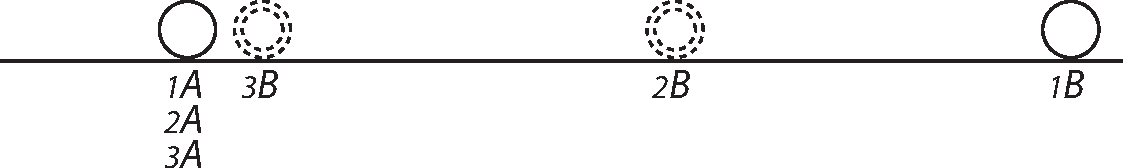
\includegraphics[width=0.75\textwidth]{%
gesamttex/edit_VIII,3/images/LH_37_05_140-141,148-149_d2_140r.pdf%
}} 
\vspace{0em}
\centerline{%
\lbrack\textit{Fig.~2}\rbrack%
}
% \newpage%
\vspace{1em}
%
\pstart
%
Alia
%
utamur ratiocinatione: videtur 
%
si duae causae\protect\index{Sachverzeichnis}{causae duae indiscernibiles}
%
sint indiscernibiles ex aliquo situ seu corpore 
%
\edtext{perfecte}{\lemma{}\Bfootnote{perfecte \textit{erg.~L}}} 
%
spectatae, esse effectus etiam indiscernibiles\protect\index{Sachverzeichnis}{effectus indiscernibiles} ex eodem corpore 
%
\edtext{spectat\lbrack os\rbrack.}{%
\lemma{}%
\Bfootnote{%
spectatae %
\textit{L ändert Hrsg.}%
}}
%
Itaque si oculus\protect\index{Sachverzeichnis}{oculus} sit in corpore moto,\protect\index{Sachverzeichnis}{oculus in corpore moto} et ad aliud corpus motum vel quiescens accedente, 
%
\edtext{videtur esse}{\lemma{videtur}\Bfootnote{\textit{(1)}~idem \textit{(2)}~esse~\textit{L}}} 
%
eadem apparentia\protect\index{Sachverzeichnis}{apparentia} effectus quae foret si illud corpus in quo est oculus\protect\index{Sachverzeichnis}{oculus in corpore quiescente} plane quiesceret, totus autem appropinquationis motus\protect\index{Sachverzeichnis}{motus appropinquationis} esset in 
%
\edtext{altero. Eadem}{\lemma{altero.}\Bfootnote{\textit{(1)}~Jam \textit{(2)}~Idem \textit{(3)}~Eadem~\textit{L}}} 
%
\edtext{ergo debet}{\lemma{}\Bfootnote{ergo \textbar\ semper \textit{gestr.} \textbar\ debet~\textit{L}}} 
%
esse apparentia,\protect\index{Sachverzeichnis}{apparentia} si corpus in quo oculus\protect\index{Sachverzeichnis}{oculus} quiesceret, et si celeritas appropinquandi\protect\index{Sachverzeichnis}{celeritas appropinquandi} inter corpora in reciproca ponderum ratione\protect\index{Sachverzeichnis}{ratio reciproca} divelleretur. At in hoc casu apparentia\protect\index{Sachverzeichnis}{apparentia} erit, quod recedant eadem qua venere celeritate, seu 
%
\edtext{quod apparens celeritas\protect\index{Sachverzeichnis}{celeritas apparens}}{\lemma{quod}\Bfootnote{\textit{(1)}~apparentia \textit{(2)}~apparens celeritas~\textit{L}}} 
%
separationis\protect\index{Sachverzeichnis}{celeritas apparens separationis} eadem sit quae apparens celeritas\protect\index{Sachverzeichnis}{celeritas apparens} appropinquationis.\protect\index{Sachverzeichnis}{celeritas apparens appropinquationis} 
%
Ergo et si unum quiescat, et proinde
%
\edtext{semper; eadem erit celeritas separationis\protect\index{Sachverzeichnis}{celeritas separationis},}{\lemma{semper;}\Bfootnote{\textit{(1)}~eadem posita celeritate appropinquationis \textit{(2)}~eadem erit celeritas \textit{(a)}~appropinq \textit{(b)}~separationis,~\textit{L}}}
%
quae appropinquationis,\protect\index{Sachverzeichnis}{celeritas appropinquationis} quocunque motu corpora moveantur. 
\pend%%%
\vspace{2.0em} %%%%%%%%% Diagramm 3
\centerline{%
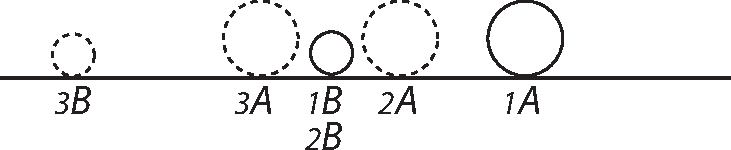
\includegraphics[width=0.55\textwidth]{%
gesamttex/edit_VIII,3/images/LH_37_05_140-141,148-149_d3_140r.pdf%
}} 
\vspace{0.5em}
\centerline{%
\lbrack\textit{Fig.~3}\rbrack%
}
% \newpage%
\vspace{1.5em}
%
\pstart
Hoc posito sumamus casum quo corpus magnum incidit in corpus parvum quiescens. 
Erit ${\scriptstyle \textit{3}}A{\scriptstyle \textit{3}}B \sqcap {\scriptstyle \textit{1}}A{\scriptstyle \textit{1}}B$, et ${\scriptstyle \textit{2}}A{\scriptstyle \textit{3}}A \smallfrown \raisebox{-1.0ex}{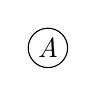
\begin{tikzpicture}\draw (0,0) circle (0.25cm) node {\textit{A}};\end{tikzpicture}} + {\scriptstyle \textit{2}}B{\scriptstyle \textit{3}}B \smallfrown \raisebox{-1.0ex}{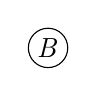
\begin{tikzpicture}\draw (0,0) circle (0.25cm) node {\textit{B}};\end{tikzpicture}} \sqcap {\scriptstyle \textit{1}}A{\scriptstyle \textit{2}}A \smallfrown \raisebox{-1.0ex}{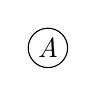
\begin{tikzpicture}\draw (0,0) circle (0.25cm) node {\textit{A}};\end{tikzpicture}} + {\scriptstyle \textit{1}}B{\scriptstyle \textit{2}}B \smallfrown %
%
%
\edlabel{37_05_140-141_2a}%
\edtext{}{% B-Footnote – Seu streicht Hrsg.
{\xxref%
{37_05_140-141_2a}{37_05_140-141_2b}}%
\lemma{}%
\Bfootnote{%
{\Large\textcircled{\protect\raisebox{0.3ex}{\footnotesize\textit{B}}}}%
. \textbar\ Seu \textit{streicht Hrsg.} \textbar\ Seu~\textit{L}%
}}%
\protect\rule[0cm]{0mm}{12pt}\raisebox{-1.0ex}{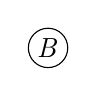
\begin{tikzpicture}\draw (0,0) circle (0.25cm) node {\textit{B}};\end{tikzpicture}}$. Seu%
\edlabel{37_05_140-141_2b}
%
$\displaystyle\frac{-{\scriptstyle \textit{2}}A{\scriptstyle \textit{3}}A+{\scriptstyle \textit{1}}A{\scriptstyle \textit{2}}A}{-{\scriptstyle \textit{1}}B{\scriptstyle \textit{2}}B+{\scriptstyle \textit{2}}B{\scriptstyle \textit{3}}B} \sqcap \displaystyle\frac{\raisebox{-1.0ex}{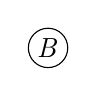
\begin{tikzpicture}\draw (0,0) circle (0.25cm) node {\textit{B}};\end{tikzpicture}}}{\raisebox{-1.0ex}{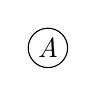
\begin{tikzpicture}\draw (0,0) circle (0.25cm) node {\textit{A}};\end{tikzpicture}}}$\rule[0mm]{0mm}{06mm}. Jam ${\scriptstyle \textit{3}}A{\scriptstyle \textit{3}}B \sqcap {\scriptstyle \textit{2}}A{\scriptstyle \textit{2}}B + {\scriptstyle \textit{2}}B{\scriptstyle \textit{3}}B - {\scriptstyle \textit{2}}A{\scriptstyle \textit{3}}A \sqcap {\scriptstyle \textit{1}}A{\scriptstyle \textit{1}}B$. Ergo ${\scriptstyle \textit{2}}B{\scriptstyle \textit{3}}B-{\scriptstyle \textit{2}}A{\scriptstyle \textit{3}}A \sqcap {\scriptstyle \textit{1}}A{\scriptstyle \textit{1}}B-{\scriptstyle \textit{2}}A{\scriptstyle \textit{2}}B.$ Ergo ${\scriptstyle \textit{2}}A{\scriptstyle \textit{3}}A \sqcap {\scriptstyle \textit{2}}B{\scriptstyle \textit{3}}B +{\scriptstyle \textit{2}}A{\scriptstyle \textit{2}}B -{\scriptstyle \textit{1}}A{\scriptstyle \textit{1}}B$ et rursus ${\scriptstyle \textit{2}}A{\scriptstyle \textit{3}}A \sqcap {\scriptstyle \textit{1}}A{\scriptstyle \textit{2}}A, +\overline{{\scriptstyle \textit{1}}B{\scriptstyle \textit{2}}B-{\scriptstyle \textit{2}}B{\scriptstyle \textit{3}}B}  \displaystyle\frac{\raisebox{-1.0ex}{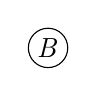
\begin{tikzpicture}\draw (0,0) circle (0.25cm) node {\textit{B}};\end{tikzpicture}}}{\raisebox{-1.0ex}{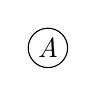
\begin{tikzpicture}\draw (0,0) circle (0.25cm) node {\textit{A}};\end{tikzpicture}}}$\rule[-4mm]{0mm}{06mm}. 
%
Ergo aequando 2 valores $ {\scriptstyle \textit{2}}B{\scriptstyle \textit{3}}B \smallfrown \raisebox{-1.0ex}{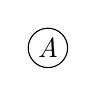
\begin{tikzpicture}\draw (0,0) circle (0.25cm) node {\textit{A}};\end{tikzpicture}} +{\scriptstyle \textit{2}}A{\scriptstyle \textit{2}}B \raisebox{-1.0ex}{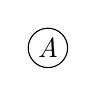
\begin{tikzpicture}\draw (0,0) circle (0.25cm) node {\textit{A}};\end{tikzpicture}} -{\scriptstyle \textit{1}}A{\scriptstyle \textit{1}}B \raisebox{-1.0ex}{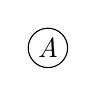
\begin{tikzpicture}\draw (0,0) circle (0.25cm) node {\textit{A}};\end{tikzpicture}} \sqcap {\scriptstyle \textit{1}}A{\scriptstyle \textit{2}}A \raisebox{-1.0ex}{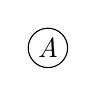
\begin{tikzpicture}\draw (0,0) circle (0.25cm) node {\textit{A}};\end{tikzpicture}} + {\scriptstyle \textit{1}}B{\scriptstyle \textit{2}}B \raisebox{-1.0ex}{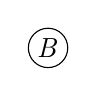
\begin{tikzpicture}\draw (0,0) circle (0.25cm) node {\textit{B}};\end{tikzpicture}} -{\scriptstyle \textit{2}}B{\scriptstyle \textit{3}}B \raisebox{-1.0ex}{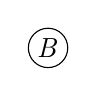
\begin{tikzpicture}\draw (0,0) circle (0.25cm) node {\textit{B}};\end{tikzpicture}}$. 
%
Ergo ${\scriptstyle \textit{2}}B{\scriptstyle \textit{3}}B \sqcap \displaystyle\frac{{\scriptstyle \textit{1}}A{\scriptstyle \textit{2}}A \raisebox{-1.0ex}{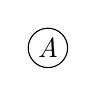
\begin{tikzpicture}\draw (0,0) circle (0.25cm) node {\textit{A}};\end{tikzpicture}} +{\scriptstyle \textit{1}}B{\scriptstyle \textit{2}}B \raisebox{-1.0ex}{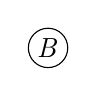
\begin{tikzpicture}\draw (0,0) circle (0.25cm) node {\textit{B}};\end{tikzpicture}} -{\scriptstyle \textit{2}}A{\scriptstyle \textit{2}}B \raisebox{-1.0ex}{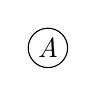
\begin{tikzpicture}\draw (0,0) circle (0.25cm) node {\textit{A}};\end{tikzpicture}} +{\scriptstyle \textit{1}}A{\scriptstyle \textit{1}}B \raisebox{-1.0ex}{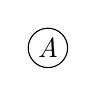
\begin{tikzpicture}\draw (0,0) circle (0.25cm) node {\textit{A}};\end{tikzpicture}}}{A+B \phantom{AAAAAAAA} {\scriptstyle \textit{2}}B{\scriptstyle \textit{3}}B}$%
\edtext{}{\lemma{\textit{{\scriptsize2}B{\scriptsize3}B}}\Cfootnote{Dieser Term im Nenner muss gestrichen werden.}}%
\rule[0mm]{0mm}{10mm}. 
%
\edtext{Si jam}{\lemma{Si}\Bfootnote{\textit{(1)}~corpora intelligantur \textit{(2)}~jam~\textit{L}}} 
%
\textit{B} quieverit et negligatur intervallum 
\protect\rule[0cm]{0mm}{12pt}\textit{{\scriptsize2}A{\scriptsize2}B}, fiet \textit{{\scriptsize2}B{\scriptsize3}B} ad \textit{{\scriptsize1}A{\scriptsize2}A} ut corpus \textit{A} duplum, ad summam 
%
\edlabel{37_05_140-141_3a}%
\edtext{}{% NEUER ABSATZ UND VARIANTEN – "utriusque. Si"
{\xxref%
{37_05_140-141_3a}{37_05_140-141_3b}}%
\lemma{utriusque.}%
\Bfootnote{%
\lbrack140~v\textsuperscript{o}\rbrack\
\textit{(1)}~\protect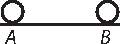
\includegraphics[width=0.1\textwidth]{%
gesamttex/edit_VIII,3/images/LH_37_05_140-141,148-149_d4_140v.pdf} \lbrack\textit{Fig.~4}\rbrack\
\textbar\ Sint \textit{streicht Hrsg.} \textbar\ corpora duo \textit{A} \textit{(2)}~Si~\textit{L}%
}}%
utriusque.
\pend
%
\pstart
\lbrack140~v\textsuperscript{o}\rbrack\ Si%
\edlabel{37_05_140-141_3b}
%
corpus unum incurrat in aliud quiescens\protect\index{Sachverzeichnis}{incursus corporis in aliud quiescens} erit celeritas quiescente accepta ad celeritatem incurrentis, ut duplum pondus\protect\index{Sachverzeichnis}{pondus} incurrentis ad summam ponderum utriusque. Hinc si corpora sint aequalia\protect\index{Sachverzeichnis}{corpora aequalia}, duplum unius aequabitur ambobus, ac proinde et celeritas 
%
\edtext{excipient\lbrack is\rbrack}{%
\lemma{excipientibus}%
\Bfootnote{%
\textit{L ändert Hrsg.}%
}}
permutabitur celeritati incurrentis. 
%
\pend 
%
\pstart 
%
Sit jam incurrens duplum excipientis 
%
\edtext{quiescentis,}{\lemma{}\Bfootnote{quiescentis \textit{erg.~L}}} 
%
\edtext{erit celeritas}{\lemma{erit}\Bfootnote{\textit{(1)}~celeritas \textit{(a)}~accepta ad \textit{(b)}~excepta ad \textit{(c)}~excipientis ad celeritatem danti \textit{(2)}~celeritas~\textit{L}}}
%
accepta ad celeritatem dantis, ut 4 (duplum incurrentis) ad 3 summam corporum. Ergo 
%
\edtext{in casu}{\lemma{in}\Bfootnote{\textit{(1)}~casu 2 erit \textit{(2)}~casu~\textit{L}}}
%
2 figurae, erit \textit{\scriptsize 2}\textit{A}\textit{\scriptsize 3}\textit{A} ad \textit{\scriptsize 1}\textit{B}\textit{\scriptsize 2}\textit{B} ut 4 
%
\edtext{ad 3. Sit}{\lemma{ad 3.}\Bfootnote{\textit{(1)}~Patebit autem eandem esse potentiam\protect\index{Sachverzeichnis}{potentia}, nam \textit{(2)}~Sit~\textit{L}}} 
%
celeritas incurrentis 
%
\edtext{3,  erit ejus}{\lemma{3, erit}\Bfootnote{\textit{(1)}~potentia accipientis \textit{(2)}~ejus~\textit{L}}} 
%
potentia 6, celeritas accipientis 4, 
%
\edtext{potentia 4. Hinc}{%
\lemma{potentia 4.}%
\Bfootnote{%
\textit{(1)}~Erit %
\textit{(2)}~Restabit %
\textit{(3)}~Hinc%
~\textit{L}%
}}
%
restabit 2 potentia ejus quod incurrerat, \edtext{ea divisa}{\lemma{ea}\Bfootnote{\textit{(1)}~est \textit{(2)}~divisa~\textit{L}}} 
%
per corpus 2, dabit 1 celeritatem qua incurrens pergit. 
%
\edtext{%	% C-Fn Verweislinie
Ergo ${\scriptstyle \textit{3}}A{\scriptstyle \textit{3}}B \sqcap 3$ ut ante, quia ${\scriptstyle \textit{2}}A{\scriptstyle \textit{3}}A \sqcap 4$ et ${\scriptstyle \textit{2}}A{\scriptstyle \textit{3}}B (\sqcap\, {\scriptstyle \textit{2}}B{\scriptstyle \textit{3}}B) \sqcap 1$, et $4-1$ est 3.}%
{\lemma{Ergo \lbrack...\rbrack\ est 3}%
\Cfootnote{%
Leibniz verweist durch einen Verbindungsstrich auf die erneute Besprechung desselben Falls, mit der dazugehörigen \lbrack\textit{Fig.~5}\rbrack, auf Bl.~141~r\textsuperscript{o} 
(S.~\refpassage{37_05_140-141_11}{37_05_140-141_11}).}} 
\pend
%
\pstart
%
Examinemus viam centri Gravitatis\protect\index{Sachverzeichnis}{via centri gravitatis} \textit{G}. Secta \textit{\scriptsize 1}\textit{A}\textit{\scriptsize 1}\textit{B} in tres partes, erit \textit{\scriptsize 1}\textit{B}\textit{\scriptsize 1}\textit{G} una tertia. 
%
Ergo via centri
%
\edtext{gravitatis\protect\index{Sachverzeichnis}{via centri gravitatis} incursu\protect\index{Sachverzeichnis}{incursus}}{\lemma{gravitatis}\Bfootnote{\textit{(1)}~per incursum \textit{(2)}~incursu~\textit{L}}} 
%
durante erit 2, rursus via centri gravitatis\protect\index{Sachverzeichnis}{via centri gravitatis} secunda \textit{\scriptsize 2}\textit{G}\textit{\scriptsize 3}\textit{G} est etiam 2. (Pono semper \textit{A} et \textit{B} esse ut puncta\protect\index{Sachverzeichnis}{punctum grave} inaequaliter gravia.) Ergo via illa est eadem. 
%
Hinc apparet calculum istum per solam regulam 
%
viae centri\protect\index{Sachverzeichnis}{regula viae centri} non fuisse satis determinatum, 
%
nam si posuissemus corpus \textit{B} incurrens quievisse, 
%
at \edtext{\lbrack\textit{A}\rbrack}{%
\lemma{}%
\Bfootnote{%
\textit{B} %
\textit{L ändert Hrsg.}%
}}
accepisse duplam prioris celeritatem quia duplo minus, tunc \textit{\scriptsize 3}\textit{G} eodem
%
foret in loco, et proinde non suffecit regula de via centri gravitatis\protect\index{Sachverzeichnis}{regula de via centri gravitatis} ad rem penitus determinandam. An forte ratio 
%
quod aequatio proveniens plures haberet radices. \pend 
%
\pstart 
%
In tertio casu sit corpus incurrens dimidium excipientis, seu incurrens 1, excipiens 2. 
%
\edtext{Celeritas excipientis}{%
\lemma{Celeritas}%
\Bfootnote{%
\textit{(1)}~incurrentis %
\textit{(2)}~excipientis%
~\textit{L}%
}}
%
erit ad celeritatem incurrentis ut duplum incurrens 2, ad summam corporum 3. 
%
Sit ergo spatium \textit{\scriptsize 1}\textit{B}\textit{\scriptsize 1}\textit{A} vel 
%
\edtext{\textit{\scriptsize 1}\textit{B}\textit{\scriptsize 2}\textit{B}, 3. Centrum}{%
\lemma{}%
\Bfootnote{%
\textit{\scriptsize 1}\textit{B}\textit{\scriptsize 2}\textit{B}, \textbar\ sit \textit{streicht Hrsg.}~\textbar\ 3. %
\textbar\ Ergo \textit{gestr.}~\textbar\
Centrum~\textit{L}}}
%
gravitatis\protect\index{Sachverzeichnis}{centrum gravitatis} seu punctum \textit{G} erit ita ut sit \textit{\scriptsize 1}\textit{A}\textit{\scriptsize 1}$G \sqcap 1$. 
%
Cumque distantia corporum\protect\index{Sachverzeichnis}{distantia corporum} debeat esse eadem quae ante, hinc \textit{\scriptsize 3}\textit{B} et
%
\textit{\scriptsize 1}\textit{G} coincident. Nam \textit{\scriptsize 2}\textit{A}\textit{\scriptsize 3}\textit{A} est 2, et \textit{\scriptsize 1}\textit{A}\textit{\scriptsize 1}\textit{G} est 1, summa 3. 
%
Via centri\protect\index{Sachverzeichnis}{via centri gravitatis} \textit{\scriptsize 1}\textit{G}\textit{\scriptsize 2}\textit{G} est 1. 
%
Cumque \textit{\scriptsize 3}\textit{A}\textit{\scriptsize 3}\textit{G} sit \protect\rule[0cm]{0mm}{16pt}$\displaystyle\frac{1}{3}$ de \textit{\scriptsize 3}\textit{A}\textit{\scriptsize 3}\textit{B}, 
%
erit etiam 1, ergo \textit{\scriptsize 2}\textit{G}\textit{\scriptsize 3}\textit{G} etiam 1, ergo rursus eadem via centri gravitatis.\protect\index{Sachverzeichnis}{via centri gravitatis} 
%
Quod si corpus parvum quievisset et 
%
\protect\rule[0cm]{0mm}{10pt}\edtext{suam potentiam\protect\index{Sachverzeichnis}{potentia}}{\lemma{suam}\Bfootnote{\textit{(1)}~celeritatem \textit{(2)}~potentiam~\textit{L}}} 
%
magno dedisset, tunc \textit{\scriptsize 2}\textit{A}\textit{\scriptsize 3}\textit{A} fuisset \protect\rule[0cm]{0mm}{16pt}$1\displaystyle\frac{1}{2}$ 
%
(seu dimidium \textit{\scriptsize 1}\textit{B}\textit{\scriptsize 2}\textit{B}), 
%
ergo \textit{\scriptsize 3}\textit{A}\textit{\scriptsize 3}\textit{G} (triens de \textit{\scriptsize 2}\textit{A}\textit{\scriptsize 3}\textit{A})
%
fuisset \protect\rule[0cm]{0mm}{16pt}$\displaystyle\frac{1}{2}$, et rursus \textit{\scriptsize 2}\textit{A}\textit{\scriptsize 3}\textit{G} fuisset 1. \protect\rule[0cm]{0mm}{10pt}Seu iterum eadem fuisset via 
%
\edtext{centri}{\lemma{}\Bfootnote{centri \textit{erg.~L}}} 
%
gravitatis.\protect\index{Sachverzeichnis}{via centri gravitatis}
%
\pend \pstart 
%
Hinc auguror elegantissima theoremata 
%
\edtext{proditura. Et}{%
\lemma{proditura.}%
\Bfootnote{%
\textit{(1)}~Item %
\textit{(2)}~Et%
~\textit{L}%
}}
%
vera forte manebit propositio
%
de via centri gravitatis\protect\index{Sachverzeichnis}{via centri gravitatis}; et demonstrabilis a posteriori 
%
ex natura corporum liberorum.\protect\index{Sachverzeichnis}{corpus liberum} Cum enim semper natura\protect\index{Sachverzeichnis}{natura} in summa lucretur, necesse est, ut libere concurrentibus 
%
corporibus\protect\index{Sachverzeichnis}{corpora libere concurrentia} 
%
aliis ascendentibus aliis descendentibus in eodem liquore,\protect\index{Sachverzeichnis}{corpora ascendentia et descendentia in liquore} eorum tamen centrum gravitatis\protect\index{Sachverzeichnis}{centrum gravitatis} vel ascendat vel 
%
descendat, vel idem maneat, quando omnia aequalia. Utile erit postea
%
tabulas motuum\protect\index{Sachverzeichnis}{tabulae motuum} calculari, et concursuum,\protect\index{Sachverzeichnis}{tabulae concursuum} 
%
\edtext{ex}{\lemma{}\Bfootnote{ex \textit{erg.~L}}} quibus elegantes poterunt duci observationes
%
per inductionem\protect\index{Sachverzeichnis}{inductio}. 
\pend 
% Zwischenüberschrift
\vspace{\baselineskip}
\pstart
\centering
\hspace{1mm}\hspace{-1mm}% Trick, weil \edlabel nicht zu \par-Beginn sein darf
\edlabel{37_05_140-141_15a}%
Nota
\pend
%
\pstart 
%
\edtext{(\protect\vphantom)Corpora mollia\protect\index{Sachverzeichnis}{corpus molle}}{\lemma{(\protect\vphantom)Corpora}\Bfootnote{\textit{(1)}~duo quae p \textit{(2)}~mollia~\textit{L}}} 
%
(seu \protect\index{Sachverzeichnis}{corpora post concursum cohaerentia}post concursum cohaerentia,) procedunt eadem celeritate quae est centri gravitatis\protect\index{Sachverzeichnis}{celeritas centri gravitatis} post 
%
\edtext{concursum. Eadem}{\lemma{concursum.}\Bfootnote{\textit{(1)}~Posito ergo centri gravitatis eandem esse viam et celeritatem ante et post concursum \textit{(2)}~Eadem~\textit{L}}}
%
procedunt via navis\protect\index{Sachverzeichnis}{via navis}\protect\index{Sachverzeichnis}{navis} sola.
%
\edtext{Ergo \protect\index{Sachverzeichnis}{via centri gravitatis}via\lbrack,\rbrack\ celeritas\protect\index{Sachverzeichnis}{celeritas centri gravitatis} et directio\protect\index{Sachverzeichnis}{directio centri gravitatis}}{\lemma{Ergo}\Bfootnote{\textit{(1)}~via \textit{(2)}~via celeritas et directio~\textit{L}}} 
%
centri gravitatis corporum mollium\protect\index{Sachverzeichnis}{corpus molle}\protect\index{Sachverzeichnis}{via centri gravitatis corporum mollium} post concursum, eadem est cum 
%
\textso{via} (id est directione et celeritate) 
%
post concursum\protect\index{Sachverzeichnis}{concursus}. At eadem est via navis\protect\index{Sachverzeichnis}{via navis} ante et 
%
post concursum. Ergo eadem est via centri gravitatis corporum mollium\protect\index{Sachverzeichnis}{via centri gravitatis corporum mollium} post concursum, quae est via navis\protect\index{Sachverzeichnis}{via navis} ante 
%
concursum seu universaliter loquendo quae est via navis. Ponendo jam viam centri gravitatis\protect\index{Sachverzeichnis}{via centri gravitatis} semper manere eandem 
%
\edtext{sequitur in corporibus mollibus\protect\index{Sachverzeichnis}{corpus molle} eam esse viam centri gravitatis\protect\index{Sachverzeichnis}{via centri gravitatis} quae est via navis\protect\index{Sachverzeichnis}{via navis}.}{%
\lemma{}%
\Afootnote{%
\textit{Neben \textup{centri gravitatis}, ohne erkennbaren Bezug:} vulgari%
}}
%
Jam ante concursum eadem est via centri 
%
\edtext{gravitatis durorum\protect\index{Sachverzeichnis}{via centri gravitatis corporum durorum}}{\lemma{gravitatis}\Bfootnote{\textit{(1)}~mollium \textit{(2)}~durorum~\textit{L}}} 
%
quae mollium.\protect\index{Sachverzeichnis}{via centri gravitatis corporum mollium} 
%
Ergo ante concursum tam in mollibus\protect\index{Sachverzeichnis}{corpus molle} quam in duris\protect\index{Sachverzeichnis}{corpus durum} eadem est via centri 
%
gravitatis\protect\index{Sachverzeichnis}{via centri gravitatis} et navis.\protect\index{Sachverzeichnis}{via navis} 
%
Ergo et post concursum, quia utrobique tam via navis\protect\index{Sachverzeichnis}{via navis}, ut patet, tam via centri\protect\index{Sachverzeichnis}{via centri gravitatis} uniformis.%
\lbrack\protect\vphantom()\rbrack%
\edlabel{37_05_140-141_15b}
%
\pend 
%
\pstart \lbrack{}141~r\textsuperscript{o}\rbrack{} 
%
Triplici via demonstrari poterunt axiomata\protect\index{Sachverzeichnis}{axioma} mea, una Metaphysica, ex eo 
%
\edtext{quia nulla}{\lemma{quia}\Bfootnote{\textit{(1)}~corpora per \textit{(2)}~nulla~\textit{L}}} 
%
ratio est, cur una apparentia\protect\index{Sachverzeichnis}{apparentia} alteri praeferatur, ergo unicuique satisfaciendum est, cum ergo secundum unam apparentiam\protect\index{Sachverzeichnis}{apparentia} 
%
\edtext{sive suppositionem (dato motu ponderibus reciproco,\protect\index{Sachverzeichnis}{motus ponderibus reciprocus})}{\lemma{}\Bfootnote{sive \lbrack...\rbrack\  reciproco,\protect\vphantom() \textit{erg.~L}}} 
%
fiat, ut corpora aequaliter recedant qua celeritate accessere, ideo idem et de caeteris 
%
\edtext{dicendum. Alia}{\lemma{dicendum.}\Bfootnote{\textit{(1)}~Idem \textit{(2)}~Alia~\textit{L}}} 
%
demonstratio ex natura 
%
centri gravitatis quod semper
%
aequaliter procedit,\protect\index{Sachverzeichnis}{centrum gravitatis semper aequaliter procedens} alia demonstratio ex natura ictus\protect\index{Sachverzeichnis}{ictus}, sed videndum ibi. 
%
Quod metaphysicos 
%
dici potest semper verum esse motum esse reciprocum ponderibus.\protect\index{Sachverzeichnis}{motus ponderibus reciprocus}
\pend
%
%
%
\vspace{1.0em} %%%%%%%%% Diagramm 5
\centerline{%
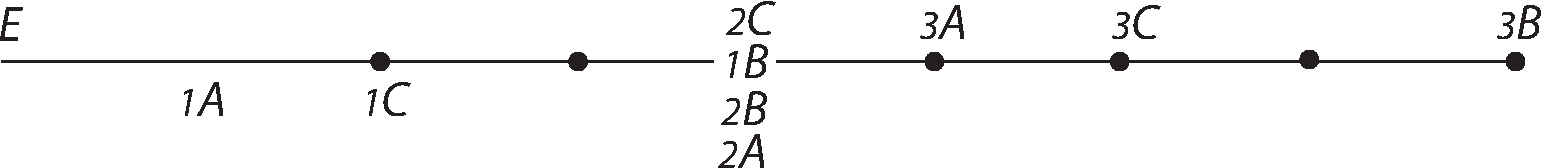
\includegraphics[width=0.9\textwidth]{%
gesamttex/edit_VIII,3/images/LH_37_05_140-141,148-149_d5_141r.pdf%
}} 
\vspace{0.5em}
\centerline{%
\lbrack\textit{Fig.~5}\rbrack%
}
% \newpage%
\vspace{1em}
%
\pstart
\hspace{1mm}\hspace{-1mm}% Trick, weil \edlabel nicht zu \par-Beginn sein darf
\edlabel{37_05_140-141_11}%
\edtext{Secundum \protect\index{Namensregister}{\textso{Huygens} (Hugenius, Ugenius, Hugens, Huguens), Christiaan 1629\textendash1695}Hugenium in hoc casu}{\lemma{Secundum \lbrack...\rbrack\ casu}%
\Cfootnote{Es handelt sich um den zehnten und letzten Fall in \protect\index{Namensregister}{\textso{Huygens} (Hugenius, Ugenius, Hugens, Huguens), Christiaan 1629\textendash1695}Huygens' Diagramm in \cite{00529}\glqq Regles du mouvement dans la rencontre des corps\grqq, \cite{00157}\textit{JS} (Pariser Ausgabe), 18.~März 1669, S.~22\textendash24 (\cite{00113}\textit{HO} XVI, S.~179\textendash181). Siehe Leibnizens kommentierte Auszüge (N.~\ref{RK57267-2}) sowie die Zusammenfassung der zehn Fälle (N.~\ref{RK60343}) von März\textendash Mai 1677.}}
%
${\scriptstyle \textit{1}}A{\scriptstyle \textit{1}}C \sqcap 1$. ${\scriptstyle \textit{1}}C{\scriptstyle \textit{1}}B \sqcap 2$. ${\scriptstyle \textit{1}}CE \sqcap 2$.\pend
%
\pstart\noindent
%
\protect\rule[0cm]{0mm}{12pt}${\scriptstyle \textit{1}}CE \sqcap {\scriptstyle \textit{1}}C$%
\raisebox{-0.7em}{$\displaystyle\left\{\efrac{{\scriptstyle \textit{2}}A}{{\scriptstyle \textit{2}}B}\right.$}%
\rule[-7mm]{0pt}{10mm}.
%
$E{\scriptstyle \textit{1}}A \sqcap {\scriptstyle \textit{2}}A{\scriptstyle \textit{3}}A.$
%
$E{\scriptstyle \textit{1}}B \sqcap {\scriptstyle \textit{2}}B{\scriptstyle \textit{3}}B$.\pend
%
\pstart\noindent
%
Ergo ${\scriptstyle \textit{1}}AE \sqcap 1$. Ergo ${\scriptstyle \textit{2}}A{\scriptstyle \textit{3}}A \sqcap 1$. 
%
$E{\scriptstyle \textit{1}}B \sqcap 4$. Ergo
%
%
\edlabel{37_05_140-141_8a}%
\edtext{}{% B-Footnote
{\xxref%
{37_05_140-141_8a}{37_05_140-141_8b}}%
\lemma{${\scriptstyle \textit{2}}B{\scriptstyle \textit{3}}B \sqcap \,4$.}\Bfootnote{\textit{(1)}~Fitque \textit{(2)}~Est~\textit{L}}}%
${\scriptstyle \textit{2}}B{\scriptstyle \textit{3}}B \sqcap 4$. 
%
\edlabel{37_05_140-141_9a}%
\edtext{}{% B-Footnote Ergänzung
{\xxref%
{37_05_140-141_9a}{37_05_140-141_9b}}%
\lemma{}%
\Bfootnote{%
Est \lbrack...\rbrack\ Hugenium \textit{erg.~L}}}%
%
Est\edlabel{37_05_140-141_8b} 
autem ${\scriptstyle \textit{3}}A{\scriptstyle \textit{2}}C \sqcap 1$. ${\scriptstyle \textit{3}}B{\scriptstyle \textit{2}}C \sqcap$ 
%
\edtext{\lbrack{}4\rbrack{}}{\lemma{2}\Bfootnote{\textit{L ändert Hrsg.}}}. 
%
\edtext{Ergo \textit{{\scriptsize2}C}\lbrack{}\textit{{\scriptsize3}C}\rbrack{} $\sqcap\, 2$ sed}%
{\lemma{}%
\Bfootnote{Ergo \textbar\ \textit{{\scriptsize2}C}\textit{{\scriptsize3}A} \textit{ändert Hrsg.} \textbar\ $\sqcap\, 2$
\textit{(1)}~ergo %
\textit{(2)}~sed%
~\textit{L}%
}} 
%
\textit{{\scriptsize1}C{\scriptsize2}C} etiam $\sqcap\, 2$. Ergo eadem via centri gravitatis\protect\index{Sachverzeichnis}{via centri gravitatis} 
%
\edtext{manet}{%
\lemma{}%
\Bfootnote{%
manet %
\textit{erg.~L}%
}}
%
apud \protect\index{Namensregister}{\textso{Huygens} (Hugenius, Ugenius, Hugens, Huguens), Christiaan 1629\textendash1695}Hugenium.\edlabel{37_05_140-141_9b}
\pend
%
\pstart\noindent
%
Etiam ${\scriptstyle \textit{1}}A{\scriptstyle \textit{1}}B \,\sqcap$ 
%
\edtext{\textit{{\scriptsize3}A{\scriptsize3}B}. Nam}{%
\lemma{\textit{{\scriptsize3}A{\scriptsize3}B}.}%
\Bfootnote{%
\textbar~Nam \textit{streicht Hrsg.}~\textbar\ %
Nam~\textit{L}}}
%
${\scriptstyle \textit{1}}A{\scriptstyle \textit{1}}B \sqcap 3$, et \textit{{\scriptsize3}A{\scriptsize3}B} 
%
$\sqcap\, 3$.
%
\pend 
%
\pstart
%
In hoc ergo \protect\index{Sachverzeichnis}{principium ejusdem distantiae}principio distantiae ejusdem, et viae
%
\edtext{centri\protect\index{Sachverzeichnis}{principium viae centri} consentit}{\lemma{centri}\Bfootnote{\textit{(1)}~manet eadem ipsi \textit{(2)}~consentit~\textit{L}}} 
%
nobiscum sed non servat eandem potentiam,\protect\index{Sachverzeichnis}{potentia}
%
\edtext{nam: posito}{\lemma{nam:}\Bfootnote{\textit{(1)}~potentia \textit{(2)}~posito~\textit{L}}}
%
corpus \textit{A} esse 2, et corpus \textit{B} esse 1, celeritas\protect\index{Sachverzeichnis}{celeritas} ipsius \textit{A} 
%
\edtext{seu \textit{{\scriptsize1}A{\scriptsize2}A}}{\lemma{}\Bfootnote{seu \textit{{\scriptsize1}A{\scriptsize2}A} \textit{erg.~L}}} 
%
est 3, celeritas ipsius \textit{B} est 0. Ergo potentia\protect\index{Sachverzeichnis}{potentia} est 6 ante concursum\protect\index{Sachverzeichnis}{concursus}. Sed
%
\edtext{post concursum\protect\index{Sachverzeichnis}{concursus} ipsius \textit{A} celeritas \textit{{\scriptsize2}A{\scriptsize3}A}}{\lemma{post concursum}\Bfootnote{\textit{(1)}~potentia \textit{(2)}~ipsius \textit{A} celeritas \textit{(a)}~est \textit{(b)}~\textit{{\scriptsize2}A{\scriptsize3}A}~\textit{L}}}
%
est 1, adeoque ejus potentia\protect\index{Sachverzeichnis}{potentia} est 2, ipsius vero \textit{B} celeritas est 4, magnitudo 1. 
%
Ergo potentia\protect\index{Sachverzeichnis}{potentia} 4. Fit ergo potentia\protect\index{Sachverzeichnis}{potentia}, 6. Hoc ergo casu non 
%
\edtext{differt calculus}{%
\lemma{differt}%
\Bfootnote{%
\textit{(1)}~casus %
\textit{(2)}~calculus%
~\textit{L}%
}}
%
\protect\index{Namensregister}{\textso{Huygens} (Hugenius, Ugenius, Hugens, Huguens), Christiaan 1629\textendash1695}Hugenii 
%
a nostro. %
\pend
%
\pstart
%
\hspace{1mm}\hspace{-1mm}% Trick, weil \edlabel nicht zu \par-Beginn sein darf
\edlabel{37_05_140-141_7a}%
\edtext{}{% C-Footnote Einfügung
{\xxref%
{37_05_140-141_7a}{37_05_140-141_6b}}%
\lemma{${\scriptstyle \textit{1}}A{\scriptstyle \textit{1}}C \sqcap bl$. \lbrack...\rbrack\ $A\;\groesser\,B$}%
\Cfootnote{%
Leibniz hat durch einen Strich, der zugleich als Einfügungszeichen dient, die ursprüngliche Fortsetzung der Passage (S.~\refpassage{37_05_140-141_6a}{37_05_140-141_6b}) von den nachträglich ergänzten Fallbesprechungen (S.~\refpassage{37_05_140-141_7a}{37_05_140-141_7b}) abgetrennt.}}%
%
\edtext{}{% B-Footnote Ergänzung
{\xxref%
{37_05_140-141_7a}{37_05_140-141_7b}}%
\lemma{}%
\Bfootnote{%
${\scriptstyle \textit{1}}A{\scriptstyle \textit{1}}C \sqcap bl$. \lbrack...\rbrack\ manet.
\textit{erg.~L}%
}}%
%
${\scriptstyle \textit{1}}A{\scriptstyle \textit{1}}C \sqcap bl$. ${\scriptstyle \textit{1}}B{\scriptstyle \textit{1}}C \sqcap al$.
${\scriptstyle \textit{1}}A{\scriptstyle \textit{2}}A \sqcap bl+al$.
%
${\scriptstyle \textit{1}}C{\scriptstyle \textit{2}}C \sqcap {\scriptstyle \textit{1}}B{\scriptstyle \textit{1}}C \sqcap al \sqcap {\scriptstyle \textit{1}}C{\scriptstyle \textit{1}}E \sqcap {\scriptstyle \textit{2}}C{\scriptstyle \textit{3}}C$.%
\pend
%
\pstart\noindent 
%
\protect\rule[0cm]{0mm}{12pt}Ergo $E{\scriptstyle \textit{1}}A \sqcap {\scriptstyle \textit{1}}C{\scriptstyle \textit{1}}E -{\scriptstyle \textit{1}}C{\scriptstyle \textit{1}}A \sqcap al-bl \sqcap {\scriptstyle \textit{2}}A{\scriptstyle \textit{3}}A$. $E{\scriptstyle \textit{1}}B \sqcap \text{bis}\ {\scriptstyle \textit{1}}C{\scriptstyle \textit{2}}C \sqcap 2al$.%
\pend
%
\pstart\noindent
%
\protect\rule[0cm]{0mm}{12pt}\edtext{${\scriptstyle \textit{1}}A{\scriptstyle \textit{3}}A\, \sqcap$ \protect\ovalbox{\textit{{\scriptsize1}A{\scriptsize1}C}} $+{\scriptstyle \textit{1}}C{\scriptstyle \textit{3}}C$\;\protect\ovalbox{$-{\scriptstyle \textit{3}}C{\scriptstyle \textit{3}}A$} $\sqcap\, 2al$ 
et ${\scriptstyle \textit{2}}A{\scriptstyle \textit{3}}A \sqcap {\scriptstyle \textit{1}}A{\scriptstyle \textit{2}}A -{\scriptstyle \textit{1}}A{\scriptstyle \textit{3}}A \,\sqcap\, \pleibdashv bl\pleibvdash al$.
${\scriptstyle \textit{2}}B{\scriptstyle \textit{3}}B\, \sqcap\, 2al$.}{%
\lemma{}%
\Bfootnote{%
${\scriptstyle \textit{1}}A{\scriptstyle \textit{3}}A\ \lbrack...\rbrack\  {\scriptstyle\textit{3}}B\, \sqcap\, 2al$. %
\textit{erg.~L}%
}}
%
\pend
%
\pstart\noindent 
Potentia\protect\index{Sachverzeichnis}{potentia} ante concursum erat $abl+a^2l$. %
%
Potentia\protect\index{Sachverzeichnis}{potentia} post concursum: $\underbrace{a^2l-abl+2abl}_{\displaystyle a^2l+abl}$\rule[-8mm]{0mm}{12mm}\,, manet ergo potentia\protect\index{Sachverzeichnis}{potentia} eadem quae ante, hoc casu.
Igitur in casu quietis alterius corporis semper 
\protect\rule[0cm]{0mm}{12pt}convenimus. 
%
%
\pend
%
\vspace{1.0em} %%%%%%%%% Diagramm 6
\centerline{%
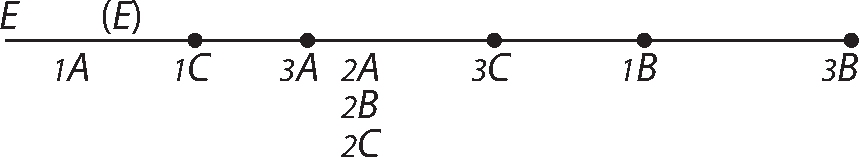
\includegraphics[width=0.6\textwidth]{%
gesamttex/edit_VIII,3/images/LH_37_05_140-141,148-149_d6_141r.pdf%
}} 
\vspace{0.5em}
\centerline{%
\lbrack\textit{Fig.~6}\rbrack%
}
% \newpage%
%
\vspace{1.0em} %%%%%%%%% Diagramm 7
\centerline{%
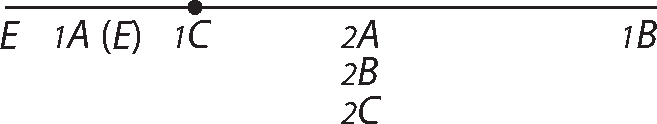
\includegraphics[width=0.47\textwidth]{%
gesamttex/edit_VIII,3/images/LH_37_05_140-141,148-149_d7_141r.pdf%
}} 
\vspace{0.5em}
\centerline{%
\lbrack\textit{Fig.~7}\rbrack%
}
% \newpage%
\vspace{1em}
%
\pstart
%
Sit celeritas corporum qua concurrunt eadem, magnitudo vero inaequalis, ${\scriptstyle \textit{1}}A{\scriptstyle \textit{1}}C \sqcap bl$, ${\scriptstyle \textit{1}}B{\scriptstyle \textit{1}}C \sqcap al$. 
%
\edtext{Celeritas tam}{\lemma{Celeritas}\Bfootnote{\textit{(1)}~utriusque \textit{(2)}~tam~\textit{L}}} 
%
unius quam alterius \rule[-4mm]{0pt}{12mm}$\displaystyle\frac{al+bl}{2} \sqcap\, 
%
\edlabel{37_05_140-141_5a}%
\edtext{}{% B-Footnote Änderung
{\xxref%
{37_05_140-141_5a}{37_05_140-141_5b}}%
\lemma{}%
\Bfootnote{%
{$\protect\overset%
{\protect\overset%
{\protect\overset%
{\displaystyle \protect\vphantom{p}\textit{{\scriptsize1}A{\scriptsize1}C}}%
{\displaystyle \protect\vphantom{p}\textit{{\scriptsize1}B{\scriptsize1}C}}}%
{\displaystyle \protect\vphantom{p}\textit{{\scriptsize1}A{\scriptsize2}A}}}%
{\textit{{\scriptsize1}B{\scriptsize2}B}}$} \; \textit{ändert Hrsg.}%
}}%
\bigg[\hspace{-0.4em}
\begin{array}{c}
\textit{{\scriptsize1}A{\scriptsize2}A}\\
\textit{{\scriptsize1}B{\scriptsize2}B}\\
\end{array}\hspace{-0.2em}\bigg]$.%
\edlabel{37_05_140-141_5b}
%
${\scriptstyle \textit{1}}C{\scriptstyle \textit{2}}C \sqcap {\scriptstyle \textit{1}}A{\scriptstyle \textit{2}}A -{\scriptstyle \textit{1}}A{\scriptstyle \textit{1}}C \sqcap \displaystyle\frac{al+bl}{2} -bl \sqcap \displaystyle\frac{al-bl}{2}$\rule[-4mm]{0pt}{12mm}. 
%
Ponamus autem corpus \textit{A} esse
%
\edtext{majus. Ergo}{\lemma{majus.}\Bfootnote{\textit{(1)}~Porro \textit{(2)}~Ergo~\textit{L}}} 
%
et ${\scriptstyle \textit{1}}CE \sqcap \displaystyle\frac{al-bl}{2}$\rule[-4mm]{0pt}{12mm}. 
%
Ergo ${\scriptstyle \textit{1}}C{\scriptstyle \textit{1}}A \sqcap {\scriptstyle \textit{1}}CE\,\pleibdashv$
%
\edtext{\textit{E{\scriptsize1}A}. Ergo}{\lemma{$\pleibdashv\; E{\scriptstyle \textit{1}}A$.}\Bfootnote{\textit{(1)}~(\protect\vphantom)si inaequalis \textit{(a)}~celeritas \textit{(b)}~via erit unius: $al+bl \smallfrown el$ alterius $\overline{al+bl} \smallfrown f$ \textit{(2)}~Ergo~\textit{L}}}
%
\rule[-4mm]{0pt}{12mm}$E{\scriptstyle \textit{1}}A \sqcap \displaystyle\efrac{\leibdashv {\scriptstyle \textit{1}}C{\scriptstyle \textit{1}}A}{\leibdashv bl} \displaystyle\efrac{\leibvdash {\scriptstyle \textit{1}}CE}{\leibvdash \displaystyle\frac{al}{2} \leibdashv \displaystyle\frac{bl}{2}} \,\sqcap\, %
%
\edtext{\pleibdashv \displaystyle\frac{3bl}{2} \pleibvdash \displaystyle\frac{al}{2}$. Et}{%
\lemma{$\pleibdashv \displaystyle\frac{3bl}{2} \pleibvdash \displaystyle\frac{al}{2}$.}%
\Bfootnote{%
\textit{(1)}~Ergo $ab+bl \sqcap el+fl$ %
\textit{(2)}~Et%
~\textit{L}%
}}
%
$EB \sqcap \displaystyle\frac{al-bl}{2} +al \sqcap \displaystyle\frac{3al-bl}{2}$\rule[-4mm]{0pt}{12mm}. 
%
Potentia\protect\index{Sachverzeichnis}{potentia} ante concursum\protect\index{Sachverzeichnis}{concursus}: $\displaystyle\frac{a^2l+abl}{2},+\displaystyle\frac{abl+b^2l}{2} \sqcap 
%
\edtext{l\displaystyle\frac{a^2+b^2+\lbrack2ab\rbrack}{2}$}{\lemma{}\Bfootnote{$2abl$ \textit{L ändert Hrsg.}}}%
\rule[-4mm]{0pt}{12mm}, postea: \rule[-4mm]{0pt}{12mm}$\displaystyle\frac{3bal-b^2l}{2}+\displaystyle\frac{a^2l-3bal}{2}$\rule[-4mm]{0pt}{12mm} (posito $a\, \groesser 3b$) quae non consentit priori \textlangle\textendash\textrangle. 
%
Non ergo eadem potentia manet.\edlabel{37_05_140-141_7b}
\pend
%
\pstart
\protect\rule[0cm]{0mm}{10pt}%
\edtext{\edlabel{37_05_140-141_6a}%
\protect\index{Namensregister}{\textso{Huygens} (Hugenius, Ugenius, Hugens, Huguens), Christiaan 1629\textendash1695}%
Hugenii constructio\protect\index{Sachverzeichnis}{constructio Hugenii} 
%
hunc dabit calculum generalem:}%
{\lemma{Hugenii \lbrack...\rbrack\ generalem}%
\Cfootnote{%
\cite{00529}a.a.O., §4, S.~22f. Leibniz bietet in N.~\ref{RK57267-2} und N.~\ref{RK60343} eine algebraische Formalisierung von \protect\index{Namensregister}{\textso{Huygens} (Hugenius, Ugenius, Hugens, Huguens), Christiaan 1629\textendash1695}Huygens' Regel.}}
\pend
%
\pstart\noindent
\rule[0cm]{0mm}{16pt}$A{\scriptstyle \textit{1}}C \sqcap bl$\hspace{5mm}$B{\scriptstyle \textit{1}}C \sqcap al$\hspace{5mm}${\scriptstyle \textit{1}}A{\scriptstyle \textit{2}}A \sqcap e$\hspace{5mm}${\scriptstyle \textit{1}}B{\scriptstyle \textit{2}}B \sqcap f$
%
\protect\rule[0cm]{0mm}{18pt}\hspace{5mm}$\displaystyle\efrac{{\scriptstyle \textit{1}}C{\scriptstyle \textit{2}}C}{{\scriptstyle \textit{1}}C{\scriptstyle \textit{2}}E} \sqcap \displaystyle\frac{ae-bf}{a+b}$\; 
%
\edtext{si $A\;\groesser\,B$.}{%
\lemma{}%
\Bfootnote{%
si $A\;\groesser\;B$. %
\textit{erg.~L}%
}}%
\edlabel{37_05_140-141_6b}
\pend
%
\pstart 
%
\lbrack141~v\textsuperscript{o}\rbrack\ 
%
\edlabel{37_05_140-141_12a}%	Referenz
\rule[-4mm]{0pt}{10mm}$\displaystyle\frac{+m-f}{+e-i} \overset{(1)}{\sqcap} \displaystyle\frac{(+)m^2-f^2}{\pmD\, e^2-i^2} \overset{(2)}{\sqcap} \displaystyle\frac{a}{b}$\rule[-4mm]{0pt}{10mm}. Sit $hm+hf \overset{(3)}{\sqcap} le+li$. 
%
Multiplicando aequ. 1 per 3 fiet \rule[-4mm]{0pt}{10mm}$\displaystyle\frac{hm^2-hf^2}{le^2-li^2} \sqcap  %
% B-Fn: Große Streichung
\edlabel{37_05_140-141_1a}%
\edtext{}{{\xxref{37_05_140-141_1a}{37_05_140-141_1b}}%
\lemma{$\displaystyle\frac{(+)m^2-f^2}{\pmD\, e^2-i^2}$.}%
\Bfootnote{%
\textit{(1)}~Sit $\ppmD \sqcap +$ erit $hm^2-hf^2 \sqcap (+) lm^2 -lf^2$. %
\textit{(a)}~Sit $h \,\groesser\, l$ erit 
\textit{(b)}~vel $hm^2 + lf^2 \sqcap (+) lm^2+hf^2$.
\textit{(aa)}~Si $l \,\groesser\,h$, erit $+lm^2 \,\groesser\, +$ \textlangle\textendash\textrangle l 
\textit{(bb)}~Si $h \,\groesser\, l$ erit $hf^2 \,\groesser\, lf^2$. Ergo si ad $hm^2-hf^2$ addas $hf^2$, et ad $(+) lm^2-lf^2$ addas 
\textit{(aaa)}~$hf^2$ 
\textit{(bbb)}~$lf^2$, tunc illi addes majus. 
\textit{(aaaa)}~Si aut 
\textit{(bbbb)}~Ergo ex illo aequalium fiet majus 
\textit{(aaaaa)}~ergo h 
\textit{(bbbbb)}~ergo $hm^2$\protect\ovalbox{$-hf^2+hf^2$} $\groesser\, (+) lm^2$ \protect\ovalbox{$-lf^2+lf^2$}. Ergo $h\,\groesser\, (+)l$. 
\textit{(aaaaa-a)}~Ergo si 
\textit{(aaaaa-aa)}~\textit{h} est majus quam 
\textit{(bbbbb-bb)}~\textit{l} est majus quam \textit{h} 
\textit{(aaaaa-aaa)}~erit $+ \sqcap -$ 
\textit{(aaaaa-aaaa)}~. Est autem et $h \,\groesser\, l$. Ergo
\textit{(bbbbb-bbbb)}~iterum
\textit{(bbbbb-bbb)}~seu si $m+f \,\groesser\, e+i$
\textit{(bbbbb-b)}~Unde nihil de signo concludi potest. 
\textit{(aaaaa-aa)}~Sin posito $h \,\groesser\, l$, sit 
\textit{(bbbbb-bb)}~Resumto $h \,\groesser\, l$, sit 
\mbox{\textit{(ccccc-cc)}}~Resumta aequatione: $hm^2-hf^2 \sqcap (+) lm^2-lf^2$.
\textit{(c)}~seu $hm^2 (-) lm^2 \sqcap hf^2-lf^2$. Ergo $\displaystyle\frac{m^2}{f^2} \sqcap \displaystyle\frac{h-l}{+h(-)l}$.
\textit{(aa)}~Ergo si $h\, \kleiner l$ erit 
\textit{(bb)}~Ergo si $(+)$ est + sive si $(-)$ est $-$ erit $m\sqcap f$. Ergo si $\ppmD \sqcap +$ erit $(+) \sqcap -$ ergo $\displaystyle\frac{m-f}{+e-i} \sqcap \displaystyle\frac{-m^2-f^2}{+e^2-i^2}$. Ergo $i \,\groesser\, e$. Ergo si $\ppmD \sqcap +$ erit $i \,\groesser\, e$, $f \,\groesser\, m$. Si $\ppmD \sqcap -$ erit 
\textit{(cc)}~et sit
\textit{(2)}~Si $\ppmD \sqcap\; +$ fiet:
\textit{L}}}%
\protect\rule[0cm]{0mm}{18pt}\displaystyle\frac{(+)m^2-f^2}{\pmD\, e^2-i^2}$.\rule[-4mm]{0pt}{10mm} 
\pend
%
\pstart Si $\ppmD \sqcap\; +$ fiet:\edlabel{37_05_140-141_1b}
%
\rule[-4mm]{0pt}{10mm}$\displaystyle\frac{hm^2-hf^2}{le^2-li^2} \sqcap \displaystyle\frac{(+)m^2-f^2}{\pmD\, e^2-i^2}$. 
%
Si $\ppmD \sqcap\; +$ erit $hm^2-hf^2 \sqcap (+) lm^2-lf^2$ et $hm^2 (-) lm^2 \sqcap hf^2-lf^2$. 
%
Seu \rule[-4mm]{0pt}{10mm}$\displaystyle\frac{m^2}{f^2} \sqcap \displaystyle\frac{h-l}{h(-)l}$. Ergo si $\ppmD \sqcap\; +$ et 
%
$
\underset%
{\displaystyle \textit{e} \text{ et } \textit{i}}% Unten
{\textit{f} \text{ et } \textit{m}}$
%
inaequales erit $(+) \sqcap -$.%
\edlabel{37_05_140-141_12b}
%
\pend
%
\pstart
Si 
%
\edtext{$\ppmD \sqcap\; -$ videamus}{\lemma{$\ppmD \sqcap -$}\Bfootnote{\textit{(1)}~fiet \textit{(2)}~videamus~\textit{L}}} 
%
an possit esse $(+) \sqcap +$\lbrack;\rbrack\ fiet: \rule[-4mm]{0pt}{11mm}$\displaystyle\frac{hm^2-hf^2}{le^2-li^2} \sqcap \displaystyle\frac{+m^2-f^2}{-e^2-i^2}$. 
%
Ergo: $le^2-li^2 \sqcap -he^2-hi^2$. Ergo $le^2+he^2 \sqcap li^2-hi^2$.
%
Ergo \rule[-4mm]{0pt}{10mm}$\displaystyle\frac{e^2}{i^2} \sqcap$ \rule[-4mm]{0pt}{10mm}%
\edtext{$\displaystyle\frac{l-h}{l+h}$. Quod}{\lemma{$\displaystyle\frac{l-h}{l+h}$.}\Bfootnote{\textit{(1)}~Ergo \textit{lf} \textit{(2)}~Ergo si \textit{(a)}~$l \,\groesser\, h$ \textit{(b)}~\textit{h} \textit{(3)}~Quod~\textit{L}}} 
%
est absurdum si $h \,\groesser\, l$. 
%
Ergo si $h \,\groesser\, l$\lbrack,\rbrack\
%
\edtext{seu si $e+i \;\groesser\, m+f$\lbrack,\rbrack}{\lemma{}\Bfootnote{seu si $e+i \;\groesser\, m+f$ \textit{erg.~L}}}
%
\protect\rule[0cm]{0mm}{12pt}et $\ppmD \sqcap\, -$ erit et $(+) \sqcap -$.
%
\pend
%
%
\vspace{1em} %%%%%%%%% Diagramm 8
\centerline{%
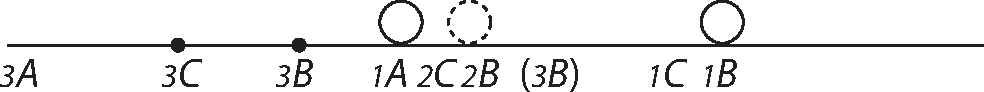
\includegraphics[width=0.7\textwidth]{%
gesamttex/edit_VIII,3/images/LH_37_05_140-141,148-149_d8_141v.pdf%
}} 
\vspace{0.5em}
\centerline{%
\lbrack\textit{Fig.~8}\rbrack}%
%
\pstart Corpus \textit{B} fertur in quiescens\protect\index{Sachverzeichnis}{corpus quiescens} \textit{A}. 
%
Centrum potentiae\protect\index{Sachverzeichnis}{centrum potentiae} 
%
\edtext{\textit{\scriptsize 1}\textit{C}}{\lemma{}\Bfootnote{\textit{\scriptsize 1}\textit{C} \textit{erg.~L}}}
%
in \textit{\scriptsize 1}\textit{B}. Erit $e \sqcap 0$, et \rule[-4mm]{0pt}{12mm}$\displaystyle\frac{a}{b} \sqcap \displaystyle\frac{m-f}{e-i} \sqcap \text{ hic } \displaystyle\frac{m-f}{-i} \sqcap \displaystyle\frac{f-m}{i}$\rule[-4mm]{0pt}{12mm} 
%
(Ergo $f \,\groesser\, m$) et $i\, \sqcap$ \rule[-4mm]{0pt}{12mm}%
\edtext{$\displaystyle\frac{b}{a}\overline{f-m}$. Jam}{\lemma{$\displaystyle\frac{b}{a}\overline{f-m}$.}\Bfootnote{\textit{(1)}~Erit a \textit{(2)}~Jam~\textit{L}}} 
%
\textit{\scriptsize 1}\textit{B}\textit{\scriptsize 2}$C\, \sqcap$ 
%
\edtext{$c \sqcap f$ seu}{\lemma{$c \sqcap f$}\Bfootnote{\textit{(1)}~Ergo \textit{(2)}~Ergo $c \sqcap f$. \textit{(3)}~seu~\textit{L}}}
%
\textit{\scriptsize 1}\textit{C}\textit{\scriptsize 2}$C \sqcap$ \rule[0cm]{0mm}{10pt}\textit{\scriptsize 1}\textit{B}\textit{\scriptsize 2}\textit{B}.
%
\pend
%
\pstart
\protect\rule[0cm]{0mm}{14pt}${\scriptstyle \textit{3}}A{\scriptstyle \textit{2}}C \sqcap$ 
%
\raisebox{-0.7em}{$\displaystyle\efrac{{\scriptstyle \textit{3}}A{\scriptstyle \textit{2}}A+{\scriptstyle \textit{2}}A{\scriptstyle \textit{2}}C}{i\phantom{AAAA} K}$}. 
%
(${\scriptstyle \textit{2}}A{\scriptstyle \textit{2}}C\sqcap {\scriptstyle \textit{2}}A{\scriptstyle \textit{2}}B \sqcap {\scriptstyle \textit{1}}A{\scriptstyle \textit{2}}B$)
%
et rursus ${\scriptstyle \textit{3}}A{\scriptstyle \textit{2}}C \sqcap {\scriptstyle \textit{3}}A{\scriptstyle \textit{3}}C+{\scriptstyle \textit{3}}C{\scriptstyle \textit{2}}C$. 
%
Ergo $i+K \sqcap {\scriptstyle \textit{3}}A{\scriptstyle \textit{3}}C+f$ seu 
%
\rule[-4mm]{0pt}{12mm}$\displaystyle\frac{b}{a}f-m +K \sqcap {\scriptstyle \textit{3}}A{\scriptstyle \textit{3}}C+f$ seu \rule[-4mm]{0pt}{12mm}$m 
%
\sqcap -\displaystyle\frac{a}{b}f-{\scriptstyle \textit{3}}A{\scriptstyle \textit{3}}C\displaystyle\frac{a}{b}+f+\displaystyle\frac{a}{b}K$\rule[-4mm]{0pt}{12mm}. 
%
Rursus ${\scriptstyle \textit{3}}B{\scriptstyle \textit{2}}C \sqcap$ \raisebox{-1.7ex}{$\displaystyle\efrac{{\scriptstyle \textit{3}}B{\scriptstyle \textit{2}}B}{m}$}$\,\sqcap\,$\raisebox{-1.7ex}{$\displaystyle\efrac{{\scriptstyle \textit{2}}C{\scriptstyle \textit{3}}C}{f}$}$-{\scriptstyle \textit{3}}C{\scriptstyle \textit{3}}B$, 
%
vel ${\scriptstyle \textit{3}}B{\scriptstyle \textit{3}}C-$\raisebox{-1.7ex}{$\displaystyle\efrac{{\scriptstyle \textit{3}}C{\scriptstyle \textit{2}}C}{f}$}. 
%
Ergo $m\, \sqcap\, \pleibdashv \,f\, \pleibvdash $\raisebox{-1.7ex}{$\displaystyle\efrac{{\scriptstyle \textit{3}}B{\scriptstyle \textit{3}}C}{\displaystyle\frac{ai}{bm}{\scriptstyle \textit{3}}A{\scriptstyle \textit{3}}C}$}. 
%
Est \rule[-4mm]{0pt}{12mm}%
\edtext{autem $\displaystyle\frac{{\scriptstyle \textit{3}}A{\scriptstyle \textit{3}}C}{{\scriptstyle \textit{3}}C{\scriptstyle \textit{3}}B}$}{\lemma{autem}\Bfootnote{\textit{(1)}~${\scriptstyle \textit{3}}A{\scriptstyle \textit{3}}C+{\scriptstyle \textit{3}}C{\scriptstyle \textit{3}}B$ ad ${\scriptstyle \textit{1}}B{\scriptstyle \textit{2}}B + {\scriptstyle \textit{1}}A{\scriptstyle \textit{2}}A$, seu ad \textit{f} ut \textit{(2)}~\textit{ib} \textit{(3)}~$\displaystyle\frac{{\scriptstyle \textit{3}}A{\scriptstyle \textit{3}}C}{{\scriptstyle \textit{3}}C{\scriptstyle \textit{3}}B}$~\textit{L}}} 
%
\edlabel{37_05_140-141_4a}%
\edtext{}{% NEUER ABSATZ UND VARIANTEN – "Via e ripa spectata"
{\xxref%
{37_05_140-141_4a}{37_05_140-141_4b}}%
\lemma{$\sqcap \displaystyle\frac{bm}{ai}.$}%
\Bfootnote{%
\textit{(1)}~Centrum gravitatis corporum absolute spectatorum, est centrum %
\textit{(2)}~Via \lbrack...\rbrack\ est 
\textbar\ eadem cum \textit{erg.}~\textbar\ %
via e ripa spectata centri~\textit{L}%
}}%
%
\edlabel{37_05_140-141_10a}%
\edtext{}{% C-Footnote Trennlinie
{\xxref%
{37_05_140-141_10a}{37_05_140-141_10b}}%
\lemma{$\displaystyle\frac{bm}{ai}.$\;\lbrack/\rbrack\;Via}%
\Cfootnote{%
Die Absätze sind durch eine waagerechte Linie getrennt.}}%
$\sqcap \displaystyle\frac{bm}{ai}.$\rule[-4mm]{0pt}{12mm}
%
\lbrack\textit{Text bricht ab.}\rbrack
\pend
%
\pstart 
\hspace{1mm}\hspace{-1mm}% Trick, weil \edlabel nicht zu \par-Beginn sein darf
\edlabel{37_05_140-141_14a}%
Via\edlabel{37_05_140-141_10b} e ripa\protect\index{Sachverzeichnis}{ripa} spectata centri gravitatis\protect\index{Sachverzeichnis}{via centri gravitatis e ripa spectata} corporum e ripa spectatorum,\protect\index{Sachverzeichnis}{corpora e ripa spectata} est eadem cum via e ripa\protect\index{Sachverzeichnis}{ripa} spectata centri%
\edlabel{37_05_140-141_4b}
%
potentiae\protect\index{Sachverzeichnis}{via centri potentiae e ripa spectata} corporum in navi\protect\index{Sachverzeichnis}{navis} 
spectatorum.\protect\index{Sachverzeichnis}{corpora in navi spectata} 
%
\edtext{Nam via centri gravitatis\protect\index{Sachverzeichnis}{via centri gravitatis} est eadem cum via navis\protect\index{Sachverzeichnis}{via navis}, 
%
ut ostendimus.}{\lemma{Nam\;\lbrack...\rbrack\;ostendimus}%
\Cfootnote{%
Siehe die ausführliche Behandlung des Stoßes anhand der Schiffsanalogie in N.~\ref{RK57269}.}}
%
\edtext{At centrum potentiae\protect\index{Sachverzeichnis}{centrum potentiae} corporum in navi spectatorum,\protect\index{Sachverzeichnis}{corpora in navi spectata}}{\lemma{At}\Bfootnote{\textit{(1)}~via centri potentiae in navi spectata \textit{(2)}~centrum potentiae corporum in navi spectatorum,~\textit{L}}}
%
ubi corpora 
%
\edtext{reciproca celeritate}{\lemma{reciproca}\Bfootnote{\textit{(1)}~potentia \textit{(2)}~celeritate~\textit{L}}} 
%
concurrunt, in navi\protect\index{Sachverzeichnis}{navis} est immobile, ergo extra spectatum movetur motu navis\protect\index{Sachverzeichnis}{navis}. 
%
Centrum potentiae\protect\index{Sachverzeichnis}{centrum potentiae} corporum in navi spectatorum\protect\index{Sachverzeichnis}{corpora in navi spectata} esset centrum ictus\protect\index{Sachverzeichnis}{centrum ictus} vel quod idem est distantiae dimidium. 
%
\pend
%
\vspace{1.0em} %%%%%%%%% Diagramm 9
\centerline{%
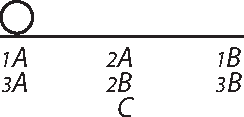
\includegraphics[width=0.25\textwidth]{%
gesamttex/edit_VIII,3/images/LH_37_05_140-141,148-149_d9_141v.pdf%
}} 
\vspace{0.2em}
\centerline{%
\lbrack\textit{Fig.~9}\rbrack%
}
% \newpage%
\vspace{1em}
%
\pstart 
%
Superest 
%
\edtext{demonstremus centrum}{\lemma{demonstremus}\Bfootnote{\textit{(1)}~centrum poten \textit{(2)}~centrum~\textit{L}}} 
%
gravitatis\protect\index{Sachverzeichnis}{centrum gravitatis} uniformiter moveri corporum distantia\protect\index{Sachverzeichnis}{distantia corporum} semper 
%
\edtext{eadem. Punctum concursus}{\lemma{eadem.}\Bfootnote{\textit{(1)}~Ergo semper punctum medium corporum eadem celeritate movetur, nisi perdatur potentia. Item \textit{(2)}~Punctum \textit{(a)}~concursum \textit{(b)}~concursus~\textit{L}}}
%
corporum in navi, est centrum gravitatis\protect\index{Sachverzeichnis}{centrum gravitatis} in distantia sumtum. 
%
Cumque semper maneat eorum centrum gravitatis\protect\index{Sachverzeichnis}{centrum gravitatis} eodem in loco in navi\protect\index{Sachverzeichnis}{navis}, quia celeritate eadem 
%
accedunt et separantur ab eo, ergo centrum gravitatis\protect\index{Sachverzeichnis}{centrum gravitatis}
%
\edtext{corporum eandem}{\lemma{corporum}\Bfootnote{\textit{(1)}~idem \textit{(a)}~manet \textit{(b)}~est \textit{(2)}~eandem~\textit{L}}} 
%
habet viam cum navi\protect\index{Sachverzeichnis}{navis}.%
\edlabel{37_05_140-141_14b}%
%
\pend
%
\pstart 
%
Constructio quaerenda. ${\scriptstyle \textit{1}}C{\scriptstyle \textit{2}}C \sqcap {\scriptstyle \textit{2}}C{\scriptstyle \textit{3}}C$ et ${\scriptstyle \textit{3}}A{\scriptstyle \textit{3}}C \sqcap {\scriptstyle \textit{1}}A{\scriptstyle \textit{1}}C$. ${\scriptstyle \textit{3}}B{\scriptstyle \textit{3}}C \sqcap {\scriptstyle \textit{1}}B{\scriptstyle \textit{1}}C$.%
%
\edtext{}{%
\lemma{\hspace*{1,6mm}%
\lbrack\textit{Fig.~10}\rbrack%
}\killnumber%
\Cfootnote{Leibniz hat den Buchstaben \textit{{\scriptsize 3}B} doppelt vergeben.}}
\pend
%
%
\vspace{1.0em} %%%%%%%%% Diagramm 10
\centerline{%
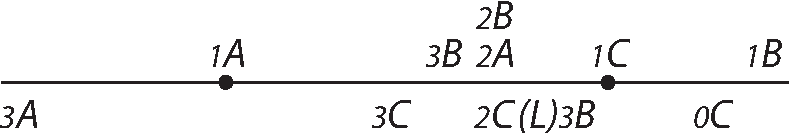
\includegraphics[width=0.55\textwidth]{%
gesamttex/edit_VIII,3/images/LH_37_05_140-141,148-149_d10_141v.pdf}} 
\vspace{0.5em}
\centerline{%
\lbrack\textit{Fig.~10}\rbrack}
%
\count\Afootins=1200%
\count\Bfootins=1200%
\count\Cfootins=1200